TODO Julie. NOTE: Use APA format.
Relevance, Likability (and Concrete/abstract)

We conducted surveys on Amazon Mechanical Turk to judge the quality of colors and palettes generated by Colorific. The study evaluated the following hypotheses:

\textbf{H1:} Machine-generated colors are perceived to be more topic-relevant than colors chosen randomly from the Protovis palette, a palette available in an industry standard data visualization toolkit. 

\textbf{H2:} Machine-generated palettes are perceived to be more likable and aesthetically pleasing than palettes composed of random Protovis colors.

\subsection{Method}
To test \textit{topic relevance}, we showed 50 participants from Mechanical Turk six options for each topic. Four of them were colors generated by Colorific. One was a random color picked from the Protovis palette, an industry standard in data visualization. The last choice was none of the above. Participants picked one choice that best suited the topic.

To test \textit{palette likability}, we wanted to test if we can combine colors from different football teams, like Cardinal, Cal Bears, and others to create a single, cohesive palette. We hypothesized that the algorithm can choose palettes that are liked better than random palettes. We weren�t sure of the best way to pick one color, so we tried four variations. One tried to pick the most frequent color, another optimized for saturation, one maximized perceptual distance between the colors, and the last picked colors from the topic at random. 
We asked 49 participants from Mechanical Turk to rate our four variations and one randomly generated palette, from Protovis on a scale of 1-7.

\subsection{Results}
\subsubsection{Topic Relevance} 
We found that the Colorific colors were preferred in an overwhelming majority ($\chi^2$ = 83.7562, df = 2, p \textless \hspace{1pt} 0.001). 947 times out of 1200, Turkers picked a Colorific color. So, Colorific is able to pick at least some good colors for a topic.

\begin{center}
\scalebox{0.15}{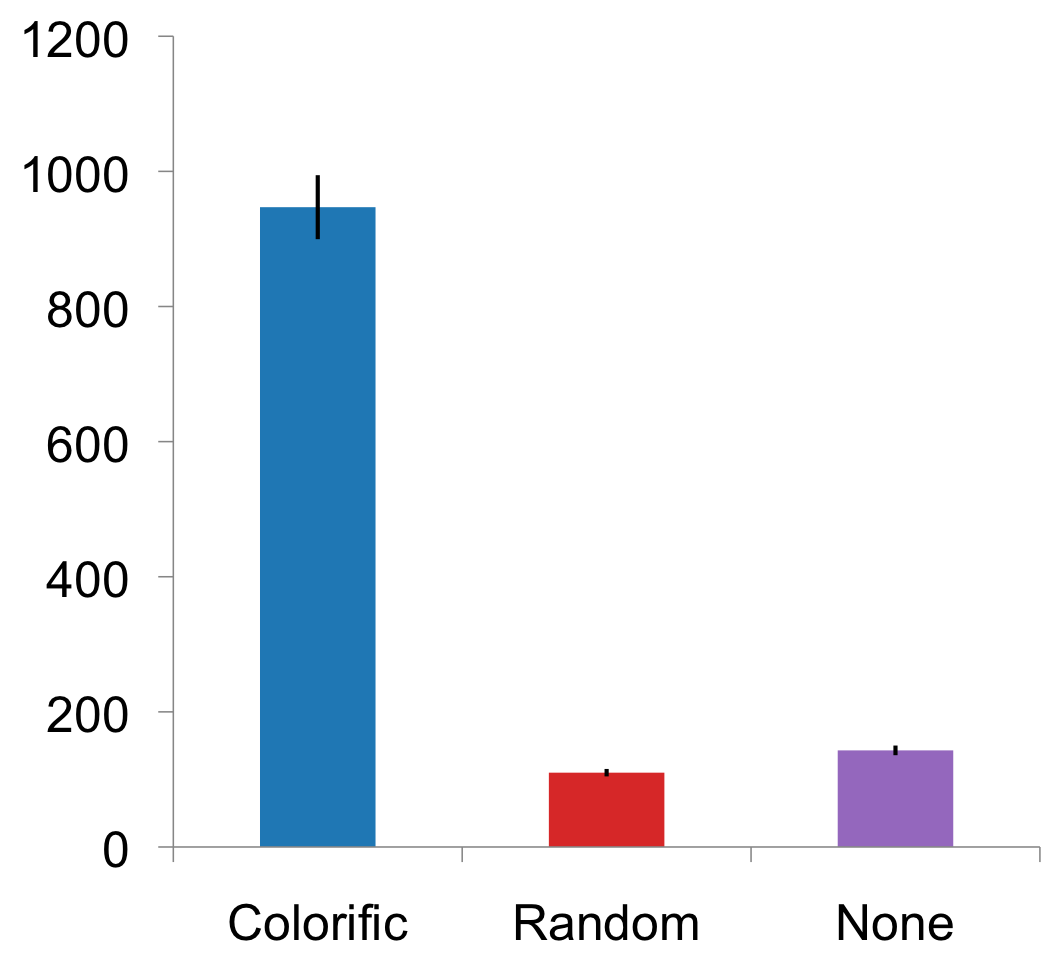
\includegraphics{relevance_chart.png}}
\end{center}

\subsubsection{Palette Likability} 
The medians of Frequency, Saturation, Distance, Random and Protovis were all 4. A Wilcoxon Signed-rank test shows that there is a significant effect of \textbf{Frequency} (W = 1, Z = -2.013, $p < 0.05$, r = -0.117) and \textbf{Distance}  (W = 1, Z = -2.431, $p < 0.05$, r = -0.142)

\begin{center}
\scalebox{0.5}{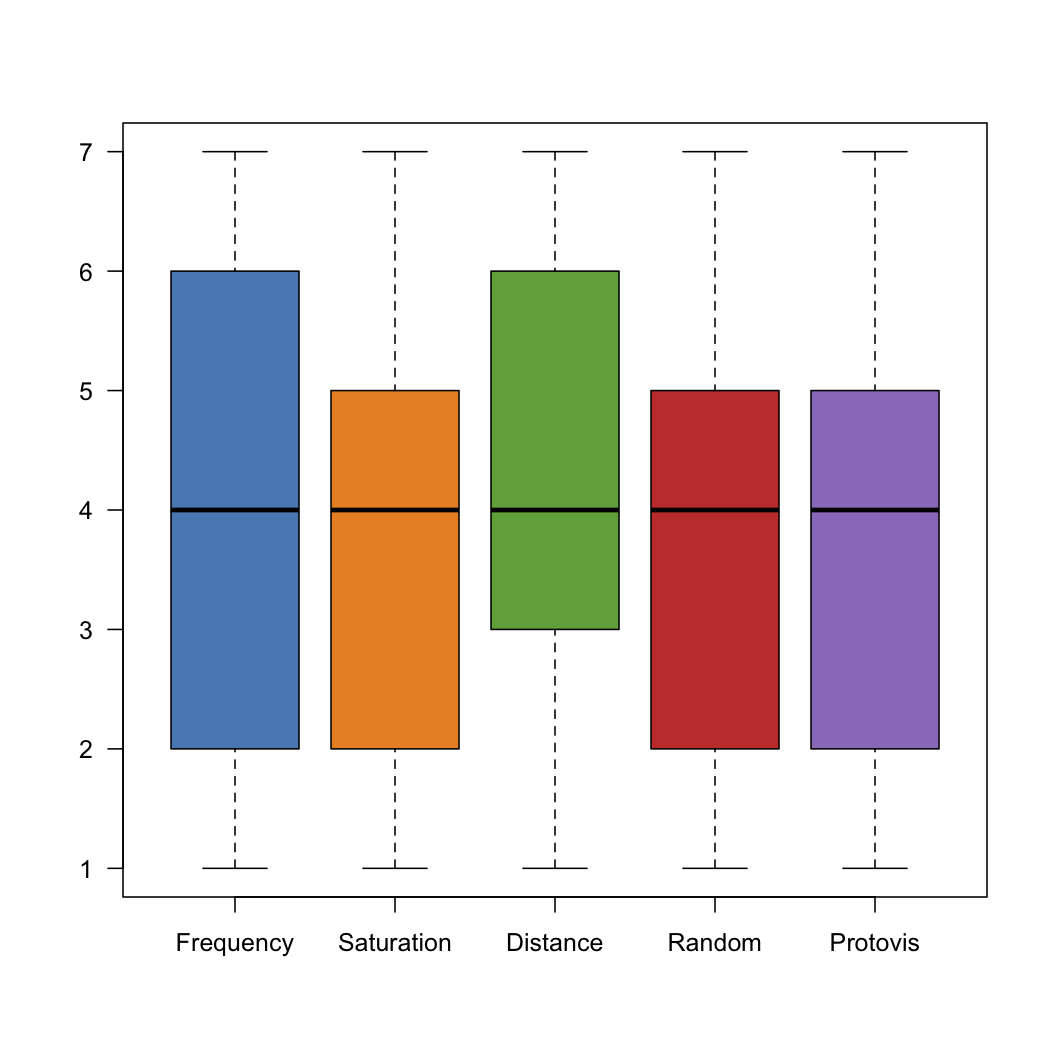
\includegraphics{likability_algorithm.png}}
\end{center}